\documentclass[10pt,a3paper,landscape]{article}

\usepackage[margin=0.9cm]{geometry}
\usepackage{graphicx}
\usepackage{xcolor}
\usepackage{multicol}
\usepackage{enumitem}
\usepackage{titlesec}
\usepackage{helvet}
\renewcommand{\familydefault}{\sfdefault}

\pagestyle{empty}
\setlength{\parindent}{0pt}
\setlength{\parskip}{0.25em}
\setlist[itemize]{leftmargin=1.1em,itemsep=0.15em,topsep=0.15em}
\titleformat{\section}{\large\bfseries\color{blue!55!black}}{}{0em}{}

\newcommand{\posterbox}[2]{%
  \fcolorbox{blue!45!black}{blue!4}{%
    \begin{minipage}{0.96\linewidth}
    \textbf{#1}\par
    #2
    \end{minipage}
  }\vspace{0.35em}
}

\begin{document}

\begin{center}
{\LARGE\bfseries In-body Antigen Detection via Antibodies on a Transistor}\\
{\large A Simulation Study of HER2 Transport, GFET Response, and Feasibility Limits}\\
\textbf{Duran Kaan Altin} \quad CMPE 492
\end{center}

\posterbox{Main finding}{Directional flow and sensor placement improve HER2 exposure, but electrostatic screening and electronics noise dominate practical GFET detectability.}

\begin{multicols}{4}

\section{Problem}
HER2 is an important breast cancer biomarker, but continuous in-body monitoring is not established. This project evaluates whether a GFET biosensor concept could detect HER2 after transport, binding, and electrical transduction are considered together.

\section{Method Pipeline}
\begin{itemize}
  \item HER2 concentration input
  \item Diffusion or prescribed directional flow
  \item Local sensor exposure
  \item Antibody binding and bound molecule count
  \item GFET current response
  \item LOD, detectability, and Debye screening tests
\end{itemize}

\section{COMSOL Model}
\begin{itemize}
  \item M2: diffusion-only Transport of Diluted Species baseline.
  \item M2B: partially anatomical prescribed-velocity convection-diffusion extension.
  \item Verification: \(v_{in}=0\) behaves like diffusion-only; increasing \(v_{in}\) changes exposure.
  \item Limitation: M2B is not a full anatomical lymph-node model and not a validated Darcy-flow pressure solution.
\end{itemize}

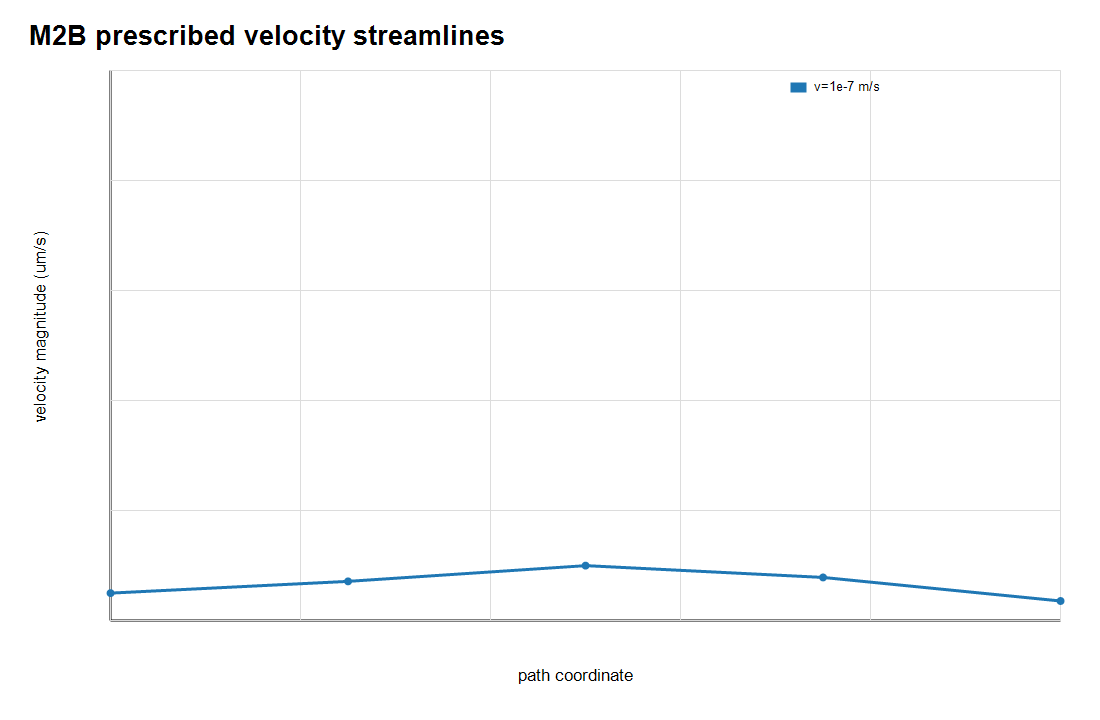
\includegraphics[width=\linewidth]{../results/figures_for_poster/M2B_flow_velocity_streamlines.png}
\textit{Prescribed M2B velocity field.}

\section{Result 1: Flow and Placement}
\begin{itemize}
  \item At \(C=10\) pM, reference flow \(v_{in}=5\times10^{-7}\) m/s gives 8.73 pM at 6000 s.
  \item Diffusion-only transport gives 4.98 pM at 6000 s.
  \item Time-to-50\% exposure decreases from about 6038 s to 1839 s.
  \item Subcapsular/cortical placement is fastest and strongest under reference flow.
\end{itemize}

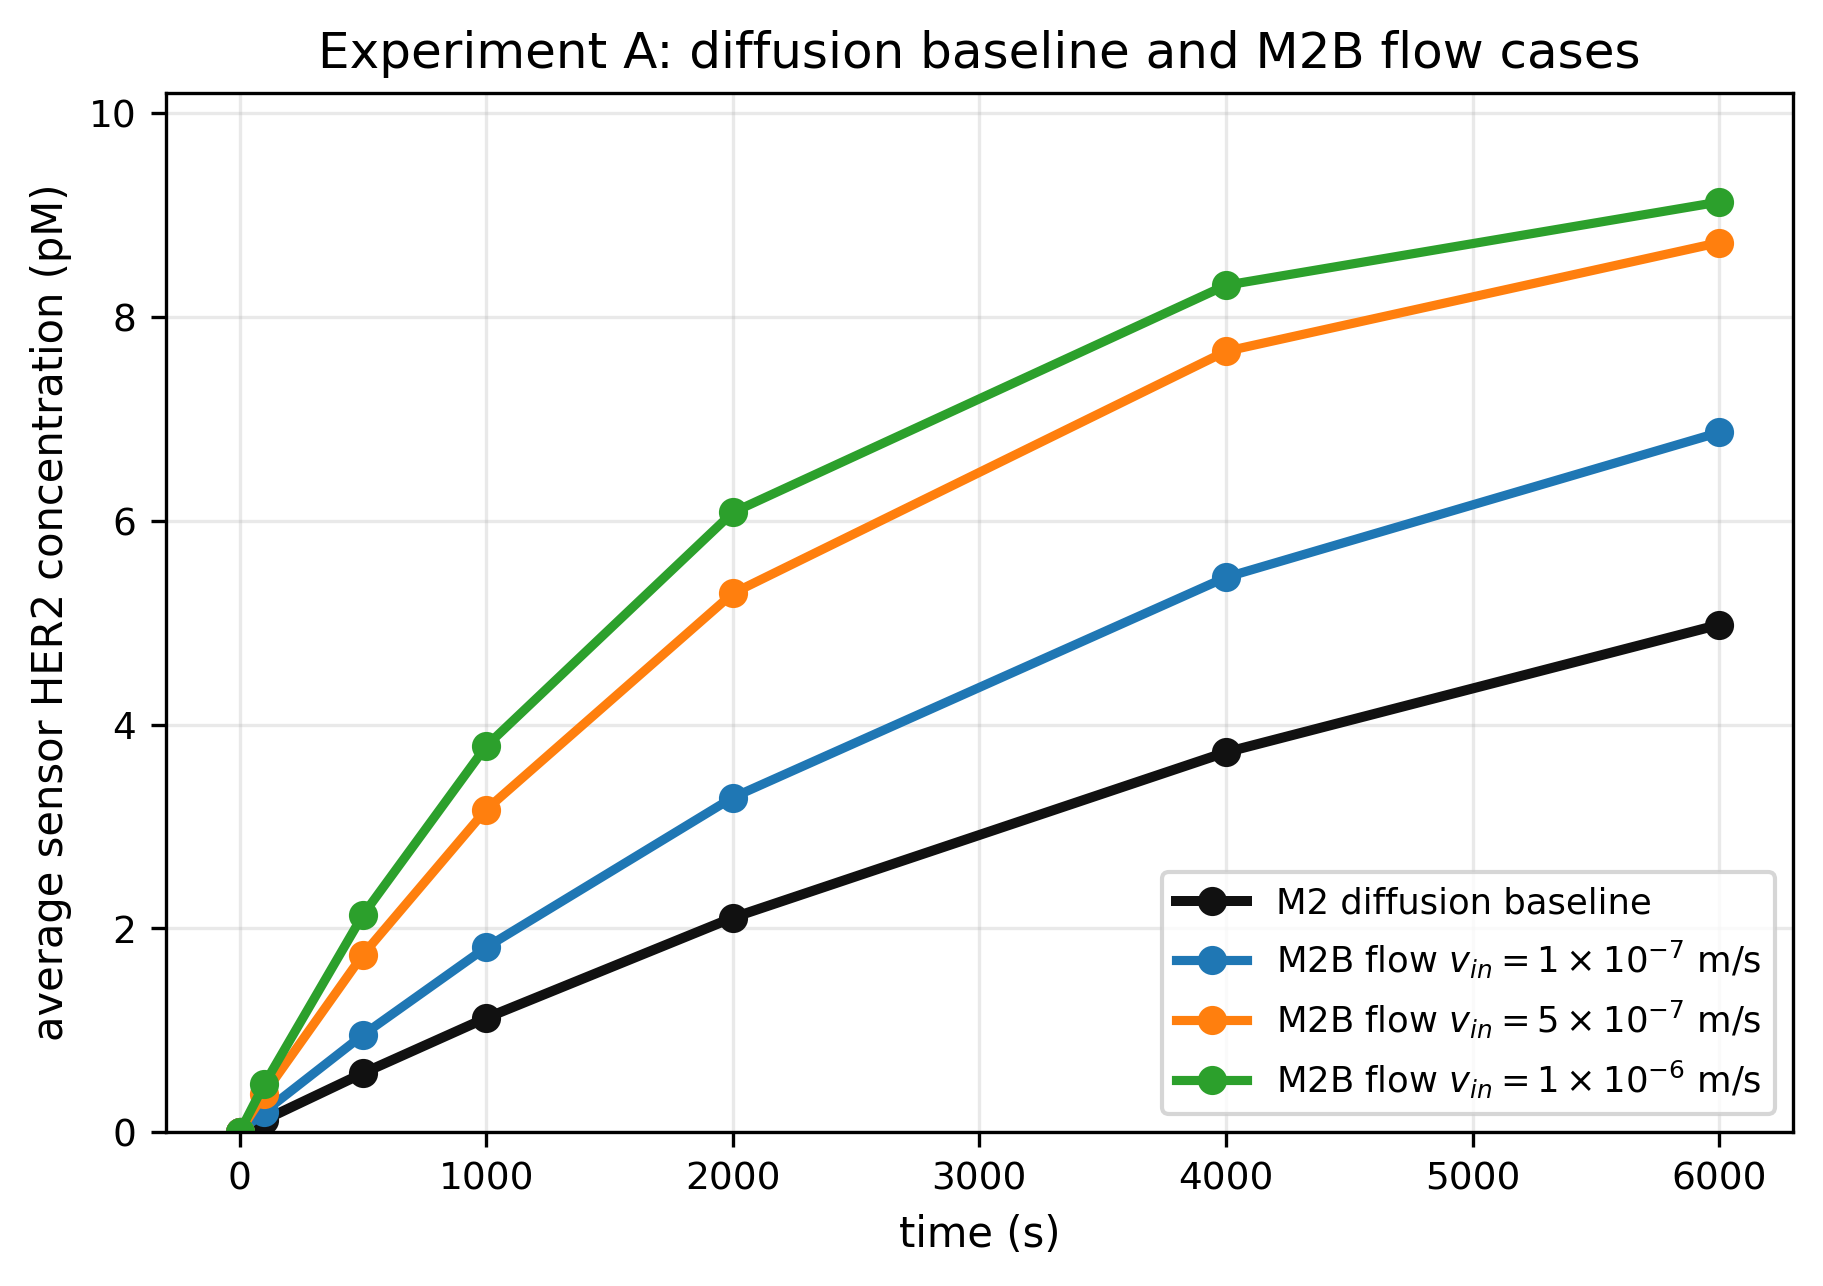
\includegraphics[width=\linewidth]{../results/figures_for_poster/EXP_A_flow_vs_diffusion_sensor_exposure.png}
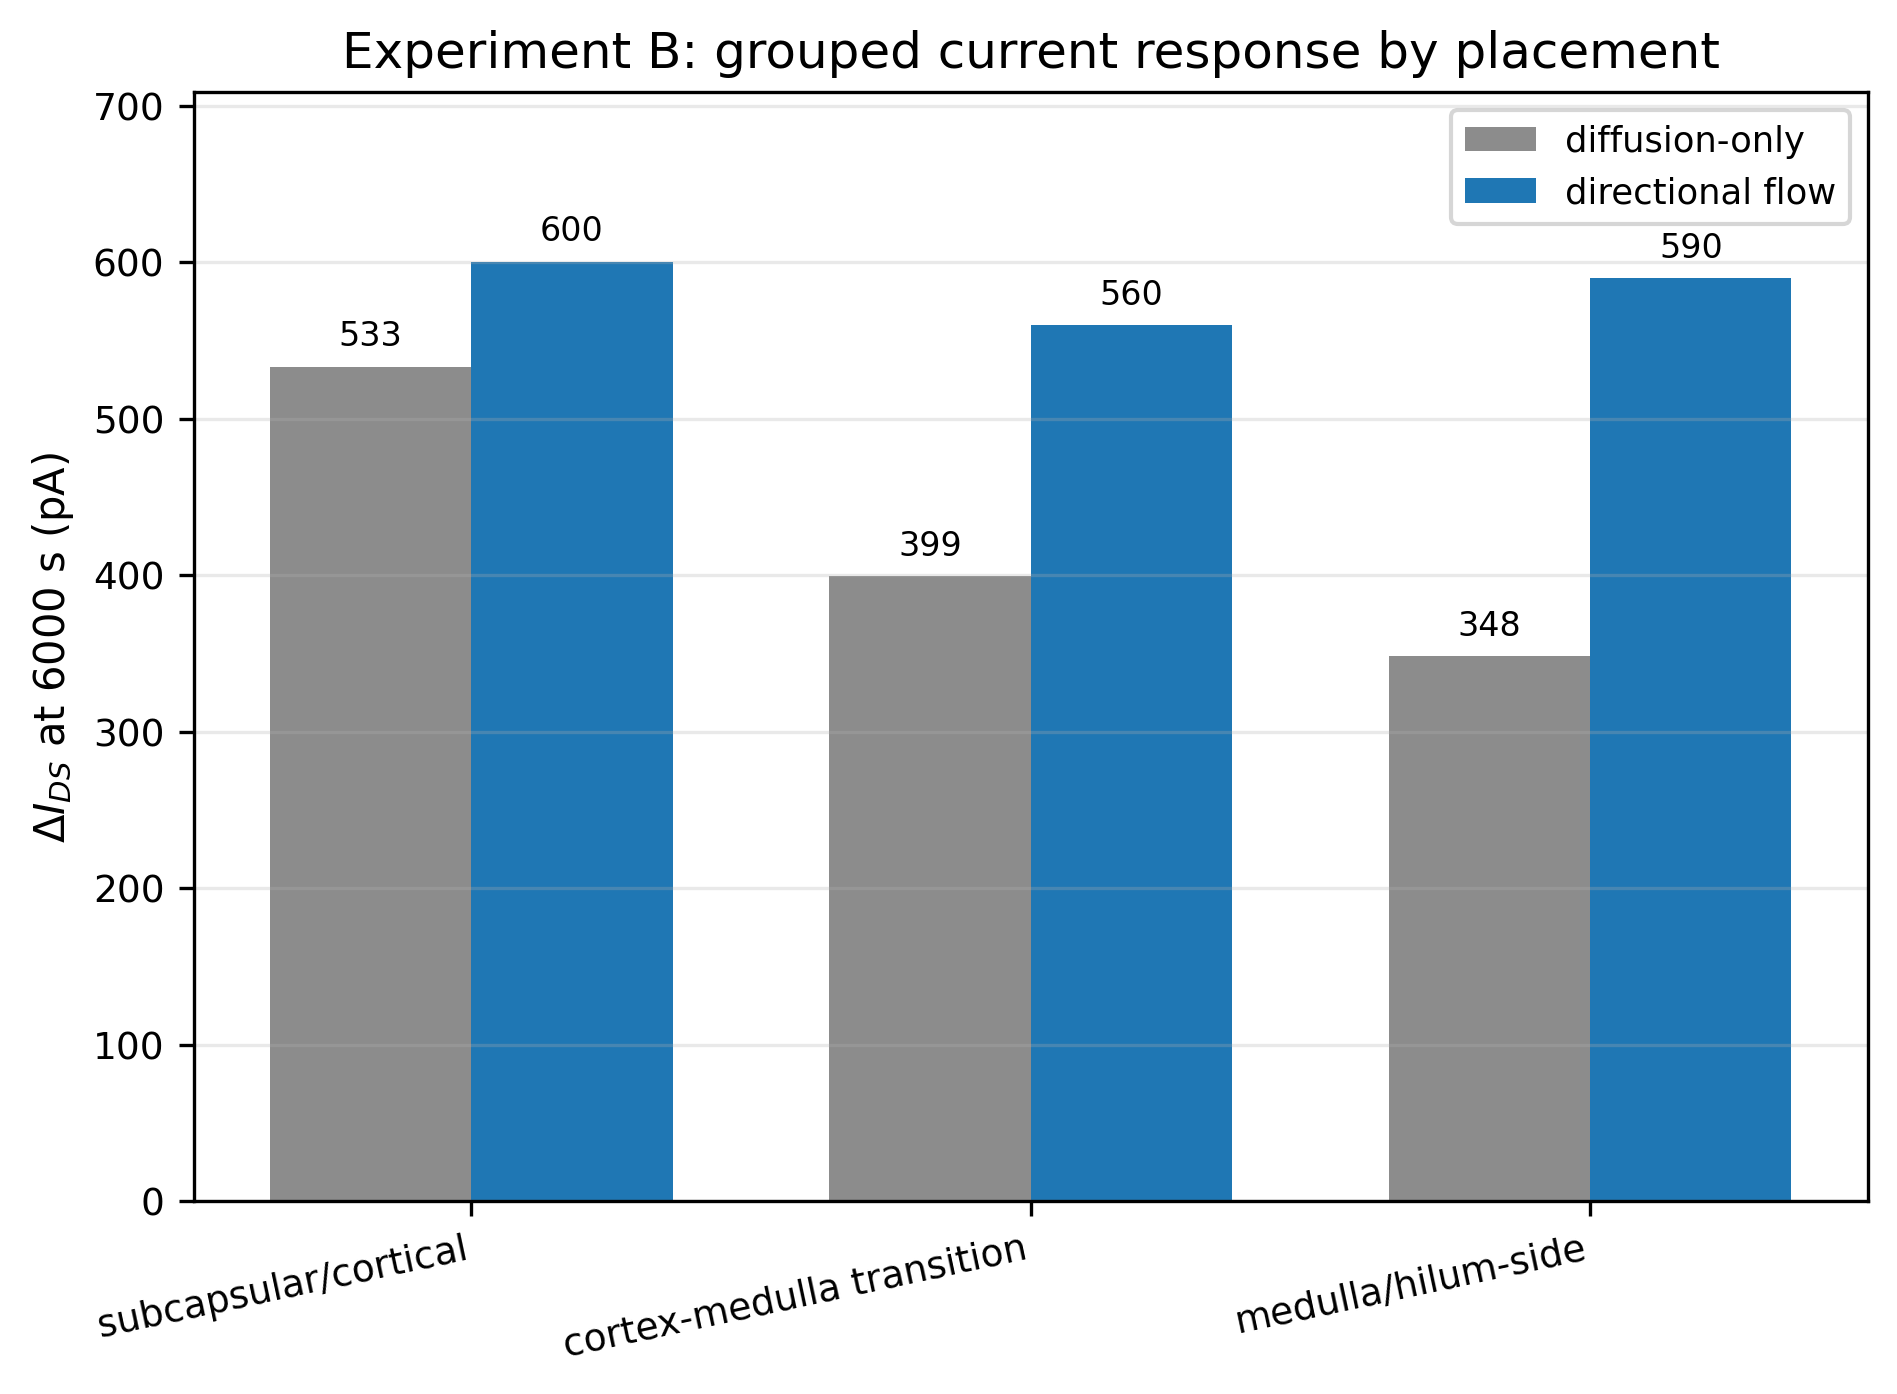
\includegraphics[width=\linewidth]{../results/figures_for_poster/EXP_B_sensor_placement_deltaIds.png}

\section{Result 2: Current Response}
\begin{itemize}
  \item GFET current response increases with HER2 concentration, coupling efficiency, and bound molecule count.
  \item Experiment C finds 99 detectable rows and 36 failing rows.
  \item Best reported M4 LOD is approximately 0.78 pM under \(\alpha=0.03\) and 10 pA noise.
  \item Sub-pM detectability is conditional, not universal.
\end{itemize}

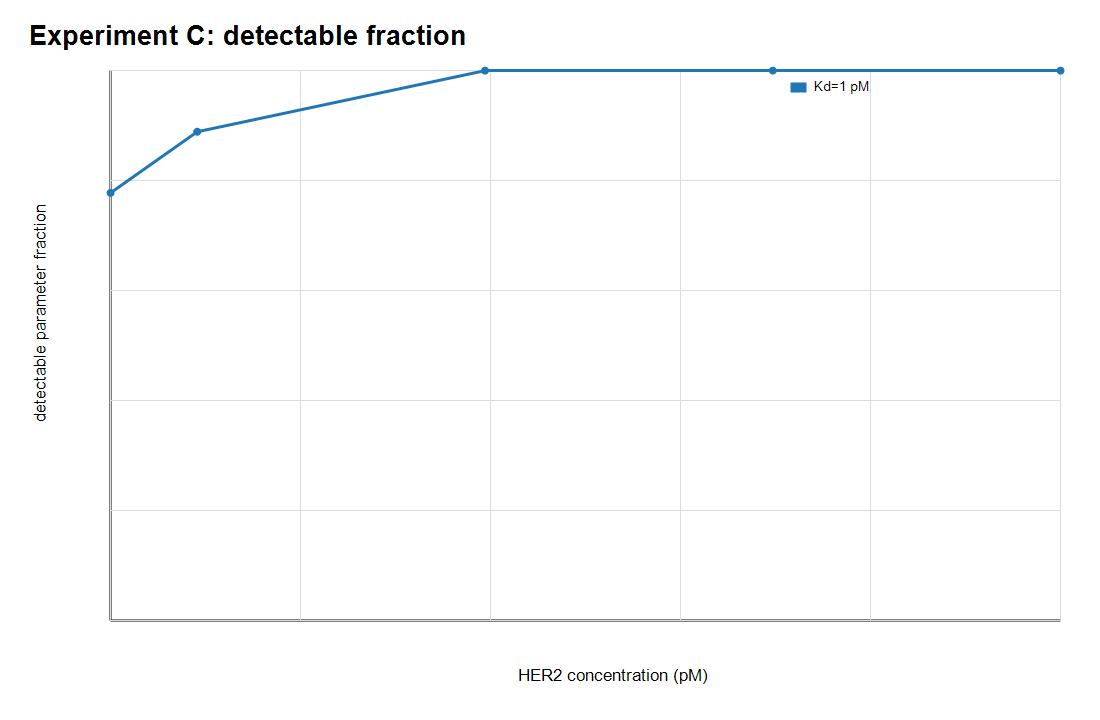
\includegraphics[width=\linewidth]{../results/figures_for_poster/EXP_C_detectable_region_map.png}

\section{Result 3: Debye Screening}
\begin{itemize}
  \item Screening uses \(\alpha_{eff}=\alpha_0\exp(-d/\lambda_D)\).
  \item PBS-like physiological salt with \(\lambda_D=0.8\) nm and \(d\geq5\) nm gives 0/60 detectable screened cases.
  \item Screening and electronics noise are the main feasibility barriers.
\end{itemize}

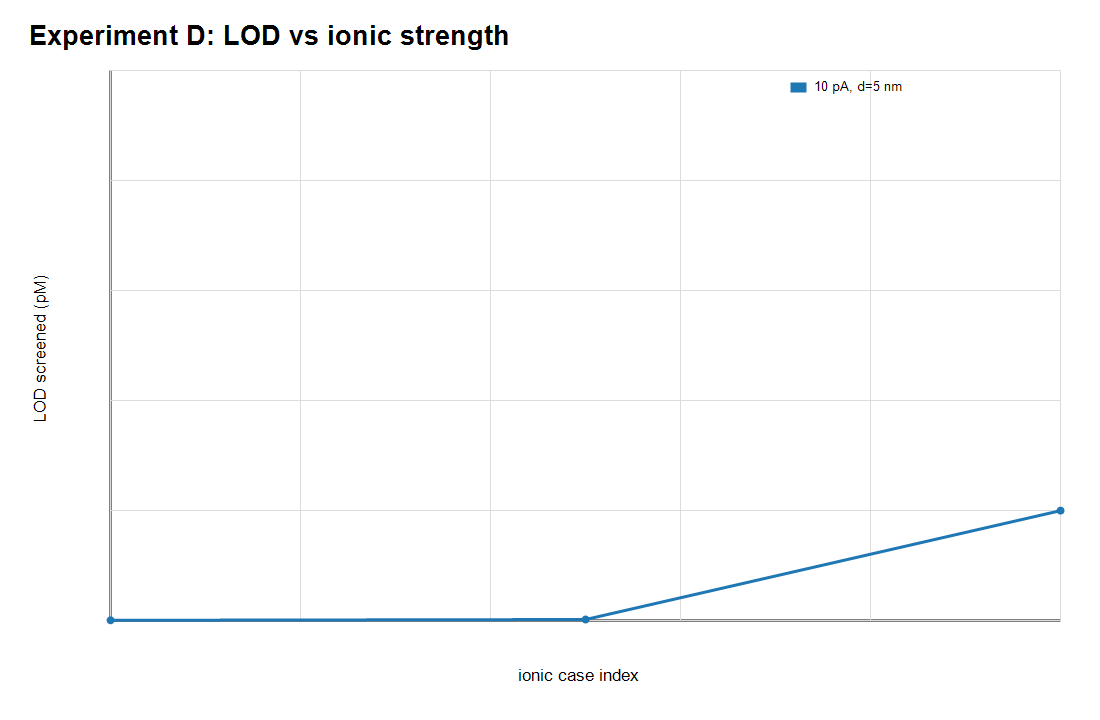
\includegraphics[width=\linewidth]{../results/figures_for_poster/EXP_D_lod_vs_ionic_strength.png}

\section{Limitations}
\begin{itemize}
  \item Simulation-only; no wet-lab or clinical validation.
  \item No fabricated device is claimed.
  \item Flow is prescribed, not a validated pressure solution.
  \item GFET response is analytical rather than a full graphene device simulation.
\end{itemize}

\section{Future Work}
\begin{itemize}
  \item Validate porous or Darcy-flow model experimentally/computationally.
  \item Automate direct COMSOL field-table export.
  \item Reduce receptor-to-channel distance.
  \item Evaluate low-noise electronics and screening mitigation.
\end{itemize}

\end{multicols}
\end{document}
